\documentclass[12pt,twoside]{article}
\usepackage{csquotes}
\usepackage{ragged2e}
\usepackage{subfig}
\usepackage{commath}

\setlength{\parindent}{4em}
\setlength{\parskip}{1em}

\newcommand{\reporttitle}{The Socioeconomic Impact of the 2012 Olympics in London.}
\newcommand{\reportauthor}{
Alp Aribal\\
Bertie Ellison-Wright\\
Pamelpreet Jhinger\\
Evonne Lee
}
\newcommand{\reportabstract}{Write an abstract summing up the report.}

% include files that load packages and define macros
%%%%%%%%%%%%%%%%%%%%%%%%%%%%%%%%%%%%%%%%%
% University Assignment Title Page 
% LaTeX Template
% Version 1.0 (27/12/12)
%
% This template has been downloaded from:
% http://www.LaTeXTemplates.com
%
% Original author:
% WikiBooks (http://en.wikibooks.org/wiki/LaTeX/Title_Creation)
%
% License:
% CC BY-NC-SA 3.0 (http://creativecommons.org/licenses/by-nc-sa/3.0/)
% 
% Instructions for using this template:
% This title page is capable of being compiled as is. This is not useful for 
% including it in another document. To do this, you have two options: 
%
% 1) Copy/paste everything between \begin{document} and \end{document} 
% starting at \begin{titlepage} and paste this into another LaTeX file where you 
% want your title page.
% OR
% 2) Remove everything outside the \begin{titlepage} and \end{titlepage} and 
% move this file to the same directory as the LaTeX file you wish to add it to. 
% Then add \input{./title_page_1.tex} to your LaTeX file where you want your
% title page.
%
%----------------------------------------------------------------------------------------
%	PACKAGES AND OTHER DOCUMENT CONFIGURATIONS
%----------------------------------------------------------------------------------------
\usepackage{ifxetex}
\usepackage{textpos}
\usepackage{natbib}
\usepackage{kpfonts}
\usepackage[a4paper,hmargin=2.8cm,vmargin=2.0cm,includeheadfoot]{geometry}
\usepackage{ifxetex}
\usepackage{stackengine}
\usepackage{tabularx,longtable,multirow,subfigure,caption}%hangcaption
\usepackage{fncylab} %formatting of labels
\usepackage{fancyhdr}
\usepackage{color}
\usepackage[tight,ugly]{units}
\usepackage{url}
\usepackage{float}
\usepackage[english]{babel}
\usepackage{amsmath}
\usepackage{graphicx}
\usepackage[colorinlistoftodos]{todonotes}
\usepackage{dsfont}
\usepackage{epstopdf} % automatically replace .eps with .pdf in graphics
\usepackage{natbib}
\usepackage{backref}
\usepackage{array}
\usepackage{latexsym}
\usepackage{etoolbox}

\usepackage{enumerate} % for numbering with [a)] format 



\ifxetex
\usepackage{fontspec}
\setmainfont[Scale=.8]{OpenDyslexic-Regular}
\else
\usepackage[pdftex,pagebackref,hypertexnames=false,colorlinks]{hyperref} % provide links in pdf
\hypersetup{pdftitle={},
  pdfsubject={}, 
  pdfauthor={\reportauthor},
  pdfkeywords={}, 
  pdfstartview=FitH,
  pdfpagemode={UseOutlines},% None, FullScreen, UseOutlines
  bookmarksnumbered=true, bookmarksopen=true, colorlinks,
    citecolor=black,%
    filecolor=black,%
    linkcolor=black,%
    urlcolor=black}
\usepackage[all]{hypcap}
\fi

\usepackage{tcolorbox}

% various theorems
\usepackage{ntheorem}
\theoremstyle{break}
\newtheorem{lemma}{Lemma}
\newtheorem{theorem}{Theorem}
\newtheorem{remark}{Remark}
\newtheorem{definition}{Definition}
\newtheorem{proof}{Proof}

% example-environment
\newenvironment{example}[1][]
{ 
\vspace{4mm}
\noindent\makebox[\linewidth]{\rule{\hsize}{1.5pt}}
\textbf{Example #1}\\
}
{ 
\noindent\newline\makebox[\linewidth]{\rule{\hsize}{1.0pt}}
}



%\renewcommand{\rmdefault}{pplx} % Palatino
% \renewcommand{\rmdefault}{put} % Utopia

\ifxetex
\else
\renewcommand*{\rmdefault}{bch} % Charter
\renewcommand*{\ttdefault}{cmtt} % Computer Modern Typewriter
%\renewcommand*{\rmdefault}{phv} % Helvetica
%\renewcommand*{\rmdefault}{iwona} % Avant Garde
\fi

\setlength{\parindent}{0em}  % indentation of paragraph

\setlength{\headheight}{14.5pt}
\pagestyle{fancy}
\fancyfoot[ER,OL]{\thepage}%Page no. in the left on
                                %odd pages and on right on even pages
\fancyfoot[OC,EC]{\sffamily }
\renewcommand{\headrulewidth}{0.1pt}
\renewcommand{\footrulewidth}{0.1pt}
\captionsetup{margin=10pt,font=small,labelfont=bf}


%--- chapter heading

\def\@makechapterhead#1{%
  \vspace*{10\p@}%
  {\parindent \z@ \raggedright %\sffamily
        %{\Large \MakeUppercase{\@chapapp} \space \thechapter}
        %\\
        %\hrulefill
        %\par\nobreak
        %\vskip 10\p@
    \interlinepenalty\@M
    \Huge \bfseries 
    \thechapter \space\space #1\par\nobreak
    \vskip 30\p@
  }}

%---chapter heading for \chapter*  
\def\@makeschapterhead#1{%
  \vspace*{10\p@}%
  {\parindent \z@ \raggedright
    \sffamily
    \interlinepenalty\@M
    \Huge \bfseries  
    #1\par\nobreak
    \vskip 30\p@
  }}
  



% %%%%%%%%%%%%% boxit
\def\Beginboxit
   {\par
    \vbox\bgroup
	   \hrule
	   \hbox\bgroup
		  \vrule \kern1.2pt %
		  \vbox\bgroup\kern1.2pt
   }

\def\Endboxit{%
			      \kern1.2pt
		       \egroup
		  \kern1.2pt\vrule
		\egroup
	   \hrule
	 \egroup
   }	

\newenvironment{boxit}{\Beginboxit}{\Endboxit}
\newenvironment{boxit*}{\Beginboxit\hbox to\hsize{}}{\Endboxit}



\allowdisplaybreaks

\makeatletter
\newcounter{elimination@steps}
\newcolumntype{R}[1]{>{\raggedleft\arraybackslash$}p{#1}<{$}}
\def\elimination@num@rights{}
\def\elimination@num@variables{}
\def\elimination@col@width{}
\newenvironment{elimination}[4][0]
{
    \setcounter{elimination@steps}{0}
    \def\elimination@num@rights{#1}
    \def\elimination@num@variables{#2}
    \def\elimination@col@width{#3}
    \renewcommand{\arraystretch}{#4}
    \start@align\@ne\st@rredtrue\m@ne
}
{
    \endalign
    \ignorespacesafterend
}
\newcommand{\eliminationstep}[2]
{
    \ifnum\value{elimination@steps}>0\leadsto\quad\fi
    \left[
        \ifnum\elimination@num@rights>0
            \begin{array}
            {@{}*{\elimination@num@variables}{R{\elimination@col@width}}
            |@{}*{\elimination@num@rights}{R{\elimination@col@width}}}
        \else
            \begin{array}
            {@{}*{\elimination@num@variables}{R{\elimination@col@width}}}
        \fi
            #1
        \end{array}
    \right]
    & 
    \begin{array}{l}
        #2
    \end{array}
    &%                                    moved second & here
    \addtocounter{elimination@steps}{1}
}
\makeatother

%% Fast macro for column vectors
\makeatletter  
\def\colvec#1{\expandafter\colvec@i#1,,,,,,,,,\@nil}
\def\colvec@i#1,#2,#3,#4,#5,#6,#7,#8,#9\@nil{% 
  \ifx$#2$ \begin{bmatrix}#1\end{bmatrix} \else
    \ifx$#3$ \begin{bmatrix}#1\\#2\end{bmatrix} \else
      \ifx$#4$ \begin{bmatrix}#1\\#2\\#3\end{bmatrix}\else
        \ifx$#5$ \begin{bmatrix}#1\\#2\\#3\\#4\end{bmatrix}\else
          \ifx$#6$ \begin{bmatrix}#1\\#2\\#3\\#4\\#5\end{bmatrix}\else
            \ifx$#7$ \begin{bmatrix}#1\\#2\\#3\\#4\\#5\\#6\end{bmatrix}\else
              \ifx$#8$ \begin{bmatrix}#1\\#2\\#3\\#4\\#5\\#6\\#7\end{bmatrix}\else
                 \PackageError{Column Vector}{The vector you tried to write is too big, use bmatrix instead}{Try using the bmatrix environment}
              \fi
            \fi
          \fi
        \fi
      \fi
    \fi
  \fi 
}  
\makeatother

\robustify{\colvec}

%%% Local Variables: 
%%% mode: latex
%%% TeX-master: "notes"
%%% End: 
 % various packages needed for maths etc.
% quick way of adding a figure
\newcommand{\fig}[3]{
 \begin{center}
 \scalebox{#3}{\includegraphics[#2]{#1}}
 \end{center}
}

%\newcommand*{\point}[1]{\vec{\mkern0mu#1}}
\newcommand{\ci}[0]{\perp\!\!\!\!\!\perp} % conditional independence
\newcommand{\point}[1]{{#1}} % points 
\renewcommand{\vec}[1]{{\boldsymbol{{#1}}}} % vector
\newcommand{\mat}[1]{{\boldsymbol{{#1}}}} % matrix
\newcommand{\R}[0]{\mathds{R}} % real numbers
\newcommand{\Z}[0]{\mathds{Z}} % integers
\newcommand{\N}[0]{\mathds{N}} % natural numbers
\newcommand{\nat}[0]{\mathds{N}} % natural numbers
\newcommand{\Q}[0]{\mathds{Q}} % rational numbers
\ifxetex
\newcommand{\C}[0]{\mathds{C}} % complex numbers
\else
\newcommand{\C}[0]{\mathds{C}} % complex numbers
\fi
\newcommand{\tr}[0]{\text{tr}} % trace
\renewcommand{\d}[0]{\mathrm{d}} % total derivative
\newcommand{\inv}{^{-1}} % inverse
\newcommand{\id}{\mathrm{id}} % identity mapping
\renewcommand{\dim}{\mathrm{dim}} % dimension
\newcommand{\rank}[0]{\mathrm{rk}} % rank
\newcommand{\determ}[1]{\mathrm{det}(#1)} % determinant
\newcommand{\scp}[2]{\langle #1 , #2 \rangle}
\newcommand{\kernel}[0]{\mathrm{ker}} % kernel/nullspace
\newcommand{\img}[0]{\mathrm{Im}} % image
\newcommand{\idx}[1]{{(#1)}}
\DeclareMathOperator*{\diag}{diag}
\newcommand{\E}{\mathds{E}} % expectation
\newcommand{\var}{\mathds{V}} % variance
\newcommand{\gauss}[2]{\mathcal{N}\big(#1,\,#2\big)} % gaussian distribution N(.,.)
\newcommand{\gaussx}[3]{\mathcal{N}\big(#1\,|\,#2,\,#3\big)} % gaussian distribution N(.|.,.)
\newcommand{\gaussBig}[2]{\mathcal{N}\left(#1,\,#2\right)} % see above, but with brackets that adjust to the height of the arguments
\newcommand{\gaussxBig}[3]{\mathcal{N}\left(#1\,|\,#2,\,#3\right)} % see above, but with brackets that adjust to the height of the arguments
\DeclareMathOperator{\cov}{Cov} % covariance (matrix) 
\ifxetex
\renewcommand{\T}[0]{^\top} % transpose
\else
\newcommand{\T}[0]{^\top}
\fi
% matrix determinant
\newcommand{\matdet}[1]{
\left|
\begin{matrix}
#1
\end{matrix}
\right|
}



%%% various color definitions
\definecolor{darkgreen}{rgb}{0,0.6,0}

\newcommand{\blue}[1]{{\color{blue}#1}}
\newcommand{\red}[1]{{\color{red}#1}}
\newcommand{\green}[1]{{\color{darkgreen}#1}}
\newcommand{\orange}[1]{{\color{orange}#1}}
\newcommand{\magenta}[1]{{\color{magenta}#1}}
\newcommand{\cyan}[1]{{\color{cyan}#1}}


% redefine emph
\renewcommand{\emph}[1]{\blue{\bf{#1}}}

% place a colored box around a character
\gdef\colchar#1#2{%
  \tikz[baseline]{%
  \node[anchor=base,inner sep=2pt,outer sep=0pt,fill = #2!20] {#1};
    }%
}%
 % short-hand notation and macros


%%%%%%%%%%%%%%%%%%%%%%%%%%%%

\begin{document}
% front page
% Last modification: 2016-09-29 (Marc Deisenroth)
\begin{titlepage}

\newcommand{\HRule}{\rule{\linewidth}{0.5mm}} % Defines a new command for the horizontal lines, change thickness here


%----------------------------------------------------------------------------------------
%	LOGO SECTION
%----------------------------------------------------------------------------------------


\includegraphics[width = 6cm]{logos/dataopen.png}\\[3.5cm]

\begin{center} % Center remainder of the page

%----------------------------------------------------------------------------------------
%	HEADING SECTIONS
%----------------------------------------------------------------------------------------
\textsc{\LARGE Summer Invitational Data Open}\\[0.5cm] 
\textsc{\Large Virtual Datathon 2020}\\[1cm]
%----------------------------------------------------------------------------------------
%	TITLE SECTION
%----------------------------------------------------------------------------------------
\HRule \\[0.4cm]
{ \huge \bfseries \reporttitle}\\ % Title of your document
\HRule \\[1.5cm]
\end{center}
%----------------------------------------------------------------------------------------
%	AUTHOR SECTION
%----------------------------------------------------------------------------------------

%\begin{minipage}{0.4\hsize}
\begin{flushleft} \large
\textit{\textbf{Team 21:}}\\
\reportauthor % Your name
\end{flushleft}
\vspace{1.5cm}
\makeatletter
Date: \@date 

\vfill % Fill the rest of the page with whitespace



\makeatother


\end{titlepage}




%%%%%%%%%%%%%%%%%%%%%%%%%%%% Main document

% Introduction
\section{Introduction}
\subsection{Background}
Hosting an Olympic games is often seen as an investment in the host city due to the increased spending infrastructure, expected boosts to tourism and the economy. Hence, due to the perceived benefits, hosting the Olympics Games became highly competitive, with many host cities promising extravagant infrastructure to secure their bids. The soaring costs, coupled with scandals in past Olympic has led to public skepticism about hosting the Olympic games. Thus, in this report, we will analyse data about Olympic host city/country, in combination with supplementary data sets, in order to increase our understanding of how hosting the Olympics has impacted the respective hosts and we will also dive into its impact on London's house pricing.\par
\subsection{Our question}
The UK stated in their bid for hosting the 2012 Olympics that they would benefit London's economy by boosting employment. We took a look at the London data sets provided relating to earnings, economic activity and infrastructure spending and found the data sets limited the scope of specific hypotheses we could hone in on.\par
After looking at supplementary data provided on \mbox{\url{https://data.london.gov.uk/}}, we found a rich data set created from the Annual Population Survey (APS), produced by the Office for National Statistics, providing data from 2004 to 2019 on the ethnicities of the working age population as well as their employment status within the UK, the major countries and regions of the UK and the London boroughs.\par
This led to the question we will investigate in this report:
\begin{displayquote}
\textbf{Did hosting the London 2012 Olympics have a lasting impact on the employment of ethnic minorities?}
\end{displayquote}
In particular, we are interested in whether the mean population and percentage employment of ethnic minorities in London has increased as a result of hosting the London 2012 Olympics.
\raggedbottom

% Technical Exposition
\section{Technical exposition}
\subsection{London House Pricing}

% Note from Pam: I moved all your figures to the appendix (just to see how much space is left).

The Mayor of London, Boris Johnson, described the area surrounding the Olympic Park as `London's single most important regeneration project for the next 25 years'. The Mayor committed to delivering sustainable economic and social development throughout east London, and closing the deprivation gap between the six Olympic host boroughs and the rest of the city. These six boroughs, Barking and Dagenham, Greenwich, Hackney, Newham, Tower Hamlets and Waltham Forest, which we will refer to as the `host boroughs' henceforth, saw significant investment into infrastructure in the years leading up to the Olympics.

We see that in 2012, these host boroughs had the 10th, 18th, 7th, 1st, 3rd and 9th highest percentages of BAME people in their population respectively compared to the other boroughs (33 in total), as shown in Fig.~\ref{fig:2012-borough-demographics}, and made up 24.6\% of the total BAME population in London, compared to 18.6\% of the general London population.

We then looked at house prices in each borough, in order to ascertain the impact of the Olympics on the cost of living in these six boroughs. In mid-2005, when London won its bid to host the Olympics, the host boroughs had the 1st, 7th, 12th, 5th, 22nd and 8th lowest house prices respectively out of all the boroughs in London, suggesting that in general, these areas were more low-income than elsewhere in the city.

Fig.~\ref{fig:house-price-percent-change-boroughs} shows the percent increase in house price from mid-2005 until 2018, with the six host boroughs shown in thick black. Fig.~\ref{fig:house-prices-percent-change-borough-map} shows the percent increase in house price from 2009 to 2015 (three years before the Olympics to three years after) on a map of London, with Olympic venues shown as pink dots, which shows how it is generally the more central boroughs that saw the greatest increase in house price. Fig.~\ref{fig:house-prices-percent-change-growth-boroughs-map} in the appendix shows the same visualisation, with only the host boroughs.

In order to determine whether the trend in change in house price was different in the host boroughs compared to the rest of London, we calculated the slope of the linear fit of the house price data between mid-2005 and 2012, and compared it to the slope of the linear fit of the data from 2012 until 2018. The slopes of the trend before and after the Olympics in each borough are shown in figures~\ref{fig:house-price-trend-before-olympics} and~\ref{fig:house-price-trend-after-olympics}.
\raggedbottom

\subsection{Employment of Ethnic Minorities}
\subsubsection{Features}
\begin{itemize}
    \item \texttt{year}: Year of observed ethnicities employed per borough.
    \item \texttt{area}: Area corresponding to where employees of a particular ethnicity reside. Includes London's boroughs, major regions of England and countries of the UK.
    \item \texttt{ethnic\_group}: Broad ethnic category in which employees fall under.
    \begin{itemize}
        \item \texttt{White}: White British and/or European.
        \item \texttt{Minority}: Total of all minority groups, including \texttt{Mixed}, \texttt{Indian}, \texttt{Black},  \texttt{Pakistani/Bangladeshi} and \texttt{Other} ethnicities. \texttt{Minority} is NOT mutually exclusive to the ethnic groups, it is a union of them all.
      \end{itemize}
    \item \texttt{number}: Number of employees (of working age) falling under the \texttt{ethnic\_group} specified working in \texttt{area}.
    \item \texttt{denominator}: Total working age population of falling under the \texttt{ethnic\_group} specified within \texttt{area}.
    \item \texttt{percent}: \texttt{number} / \texttt{denominator} i.e. the percentage of the working age population of \texttt{area} of \texttt{ethnic\_group} descent that are employed.
\end{itemize}
\subsubsection{Data manipulation}
The employment data for the major ethnic categories, white and ethnic minority, were fully populated however the specific ethnicities that the ethnic minority consisted of were not. We made the choice not to linearly interpolate this data since we were not particularly interested in a specific ethnicity's working age population, however this led to rendering line graphs that were missing points for some ethnicities.
\subsubsection{Exploratory Data Analysis}
Fig.~\ref{fig:perc-hosting} shows the percentage employment per ethnic group in the hosting Olympic boroughs and Fig.~\ref{fig:pop-hosting} shows the population employed by ethnic group within the same region. We can observe that pre-2012, the percentage employment of ethnic minorities sporadically but insignificantly changes and so stays around about the same but starts to pick up around 2012 and then continues to increase after the year of the Games.

We can also see a similar pattern in the rest of London, excluding the hosting boroughs in Fig.~\ref{fig:perc-rest-of-london} and Fig.~\ref{fig:pop-rest-of-london} where employment of ethnic minorities increased by around 10\%.

When we compare this against the employment in the rest of the UK, excluding London, in Fig.~\ref{fig:perc-uk-no-london}, we can see that, although the trend is the same, the employment of ethnic minorities only went up by around 5\%. This suggests a potential correlation between the attractiveness of London in particular within the UK, pushed through Olympic campaigns.

% Data analysis
\subsection{Hypothesis Testing}
\begin{table}[!htb]
\caption{Sample statistics generated from the employment ethnicity data.}
\label{tab:results}
\centering
\begin{tabular}{llll}
Year range & Sample mean $\overline{x}$ & Sample variance $s_{n-1}^2$ & Sample standard deviation $s_{n-1}$\\
2004 to 2011 & $1,094,012.5$ & $14,319,044,106.1$ & $119,662.2$\\
2012 to 2019 & $1,488,712.5$ & $13,553,304,106.1$ & $116,418.7$\\
\end{tabular}
\end{table}

We only have 8 samples (years) of data before 2012 and 8 samples after (and including) 2012 and we want to compare the population means of these two sets, in particular whether the population mean after 2012 was higher. This is an opportunity for a one-sided hypothesis test looking for a difference in population mean.

We shall assume that the years 2004 to 2011 and 2012 to 2019 are two independent samples of independent and identically distributed variables, the population of ethnic minorities for each year.

The Annual Population Survey is a sampled survey, therefore we do not know the true population mean before ($\mu_\text{before}$) and after ($\mu_\text{after}$) nor the true sample variance before ($s_{n-1}_\text{before}^2$) and after ($s_{n-1}_\text{after}^2$).

The null hypothesis $H_0: \mu_\text{before} = \mu_\text{after}$ for this hypothesis test is that the population mean of ethnic minorities employed in London has not changed significantly from before 2012 to after 2012.

The alternative hypothesis $H_1: \mu_\text{before} < \mu_\text{after}$ suggests that the population mean of ethnic minorities employed in London has increased significantly from before 2012 to after 2012.

We will conduct the hypothesis test with a Type I error rate of 0.01 (significance level of $1\%$) and using the Student's $t$-distribution. Using this distribution for a hypothesis test investigating for a difference in population means requires a bias-corrected sample pooled variance $s_{n_x+n_y-2}^2$.
$$s_{n_x+n_y-2}^2 = \frac{n_x-1}{n_x+n_y-2}s_{n_x-1}^2 + \frac{n_y-1}{n_x+n_y-2}s_{n_y-1}^2 = 13,936,174,106.1$$

Assuming $H_0$, applying the Student's $t$-distribution to the data along with the bias-corrected sample pooled variance gives
$$T = \frac{(\overline{X}-\overline{Y})}{s_{n_x+n_y-2}\sqrt{\frac{1}{n_x}+\frac{1}{n_y}}} \sim \Theta$$

The rejection region for the null hypothesis $H_0$ of a one-sided hypothesis test at the 10\% significance level for two population means with sample sizes 8 and 8 is
$$R=\{t\mid\abs{t}>t_{14\text{,}0.99}\}=\{t\mid\abs{t}>2.624494\}$$

The test statistic (with the appropriate parameters we have calculated inputted)
$$t=\frac{\overline{x}-\overline{y}}{s_{n_x+n_y-2}\sqrt{\frac{1}{n_x}+\frac{1}{n_y}}}=-6.686907880637657$$
We can easily see that $6.69 > 2.62$ therefore we reject the null hypothesis $H_0$ at the 1\% significance level and accept the alternative hypothesis $H_1$.

\subsection{Interpretation of Hypothesis Test Result}

The results tell us that there has been a significant increase in the population of ethnic minorities employed in London after 2012. This suggests a correlation between London hosting the Olympics  in 2012 and the increase in employment of ethnic minorities since the data used was separated into two sets dependent on the time of the Olympics.

However, we cannot ignore the fact that these results do not directly suggest a causal relationship between London hosting the 2012 Olympics and an increase in employment of ethnic minorities.

Without the pretense that the Olympics was hosted in 2012, the data itself is blind to any economic activities that have occurred since 2004. The data itself was also aggregated into records defining geographic regions, potentially losing some useful attributes such as individual reasoning for employment and whether those employed are immigrants.

Unfortunately there is not a data set available to the public that has the level of depth we are looking for, however if there was one, we believe we could prove a causal relationship between the two variables in question.

% Conclusion
%\section{Executive Summary}
% What is the question that your team set out to answer? What were your key findings, and what is their significance? You must communicate your insights clearly.
% Was the boost in employment worth the expenditure of hosting the Games.




\newpage
% Appendix
\section{Appendix}

\begin{figure}[!htb]
\centering
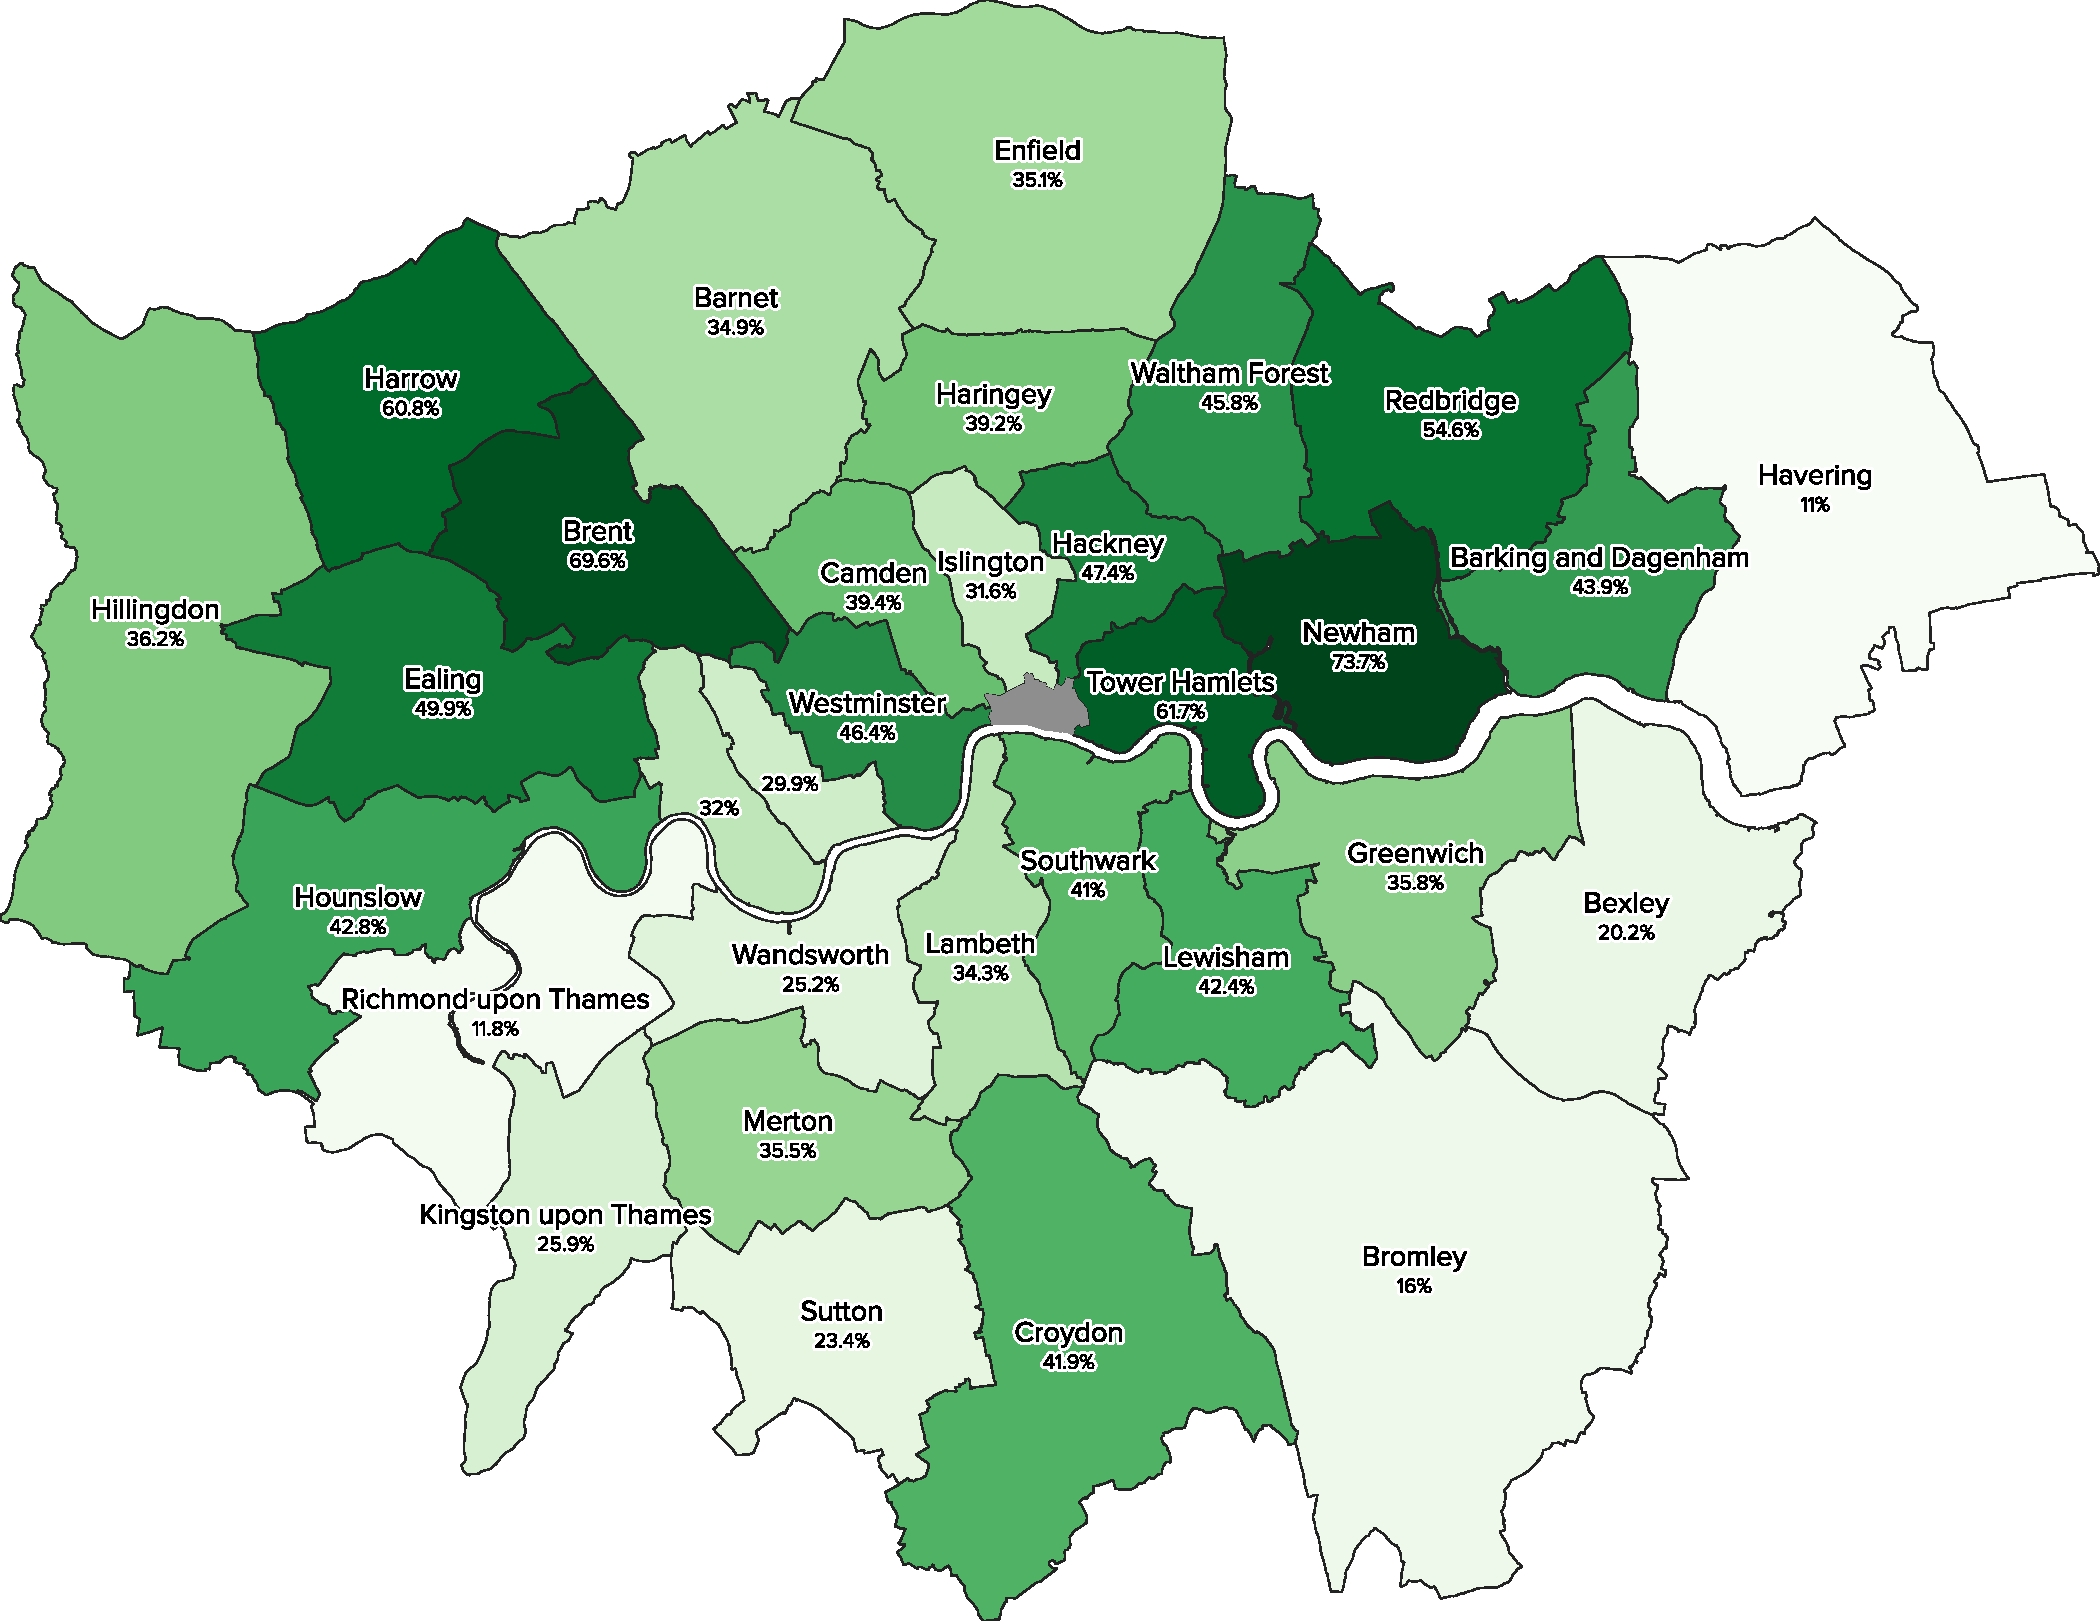
\includegraphics[width=0.8\linewidth]{figures/2012-borough-demographics.pdf}
\caption{Percentage of BAME in each borough in 2012.}
\label{fig:2012-borough-demographics}
\end{figure}

\begin{figure}[!htb]
\centering
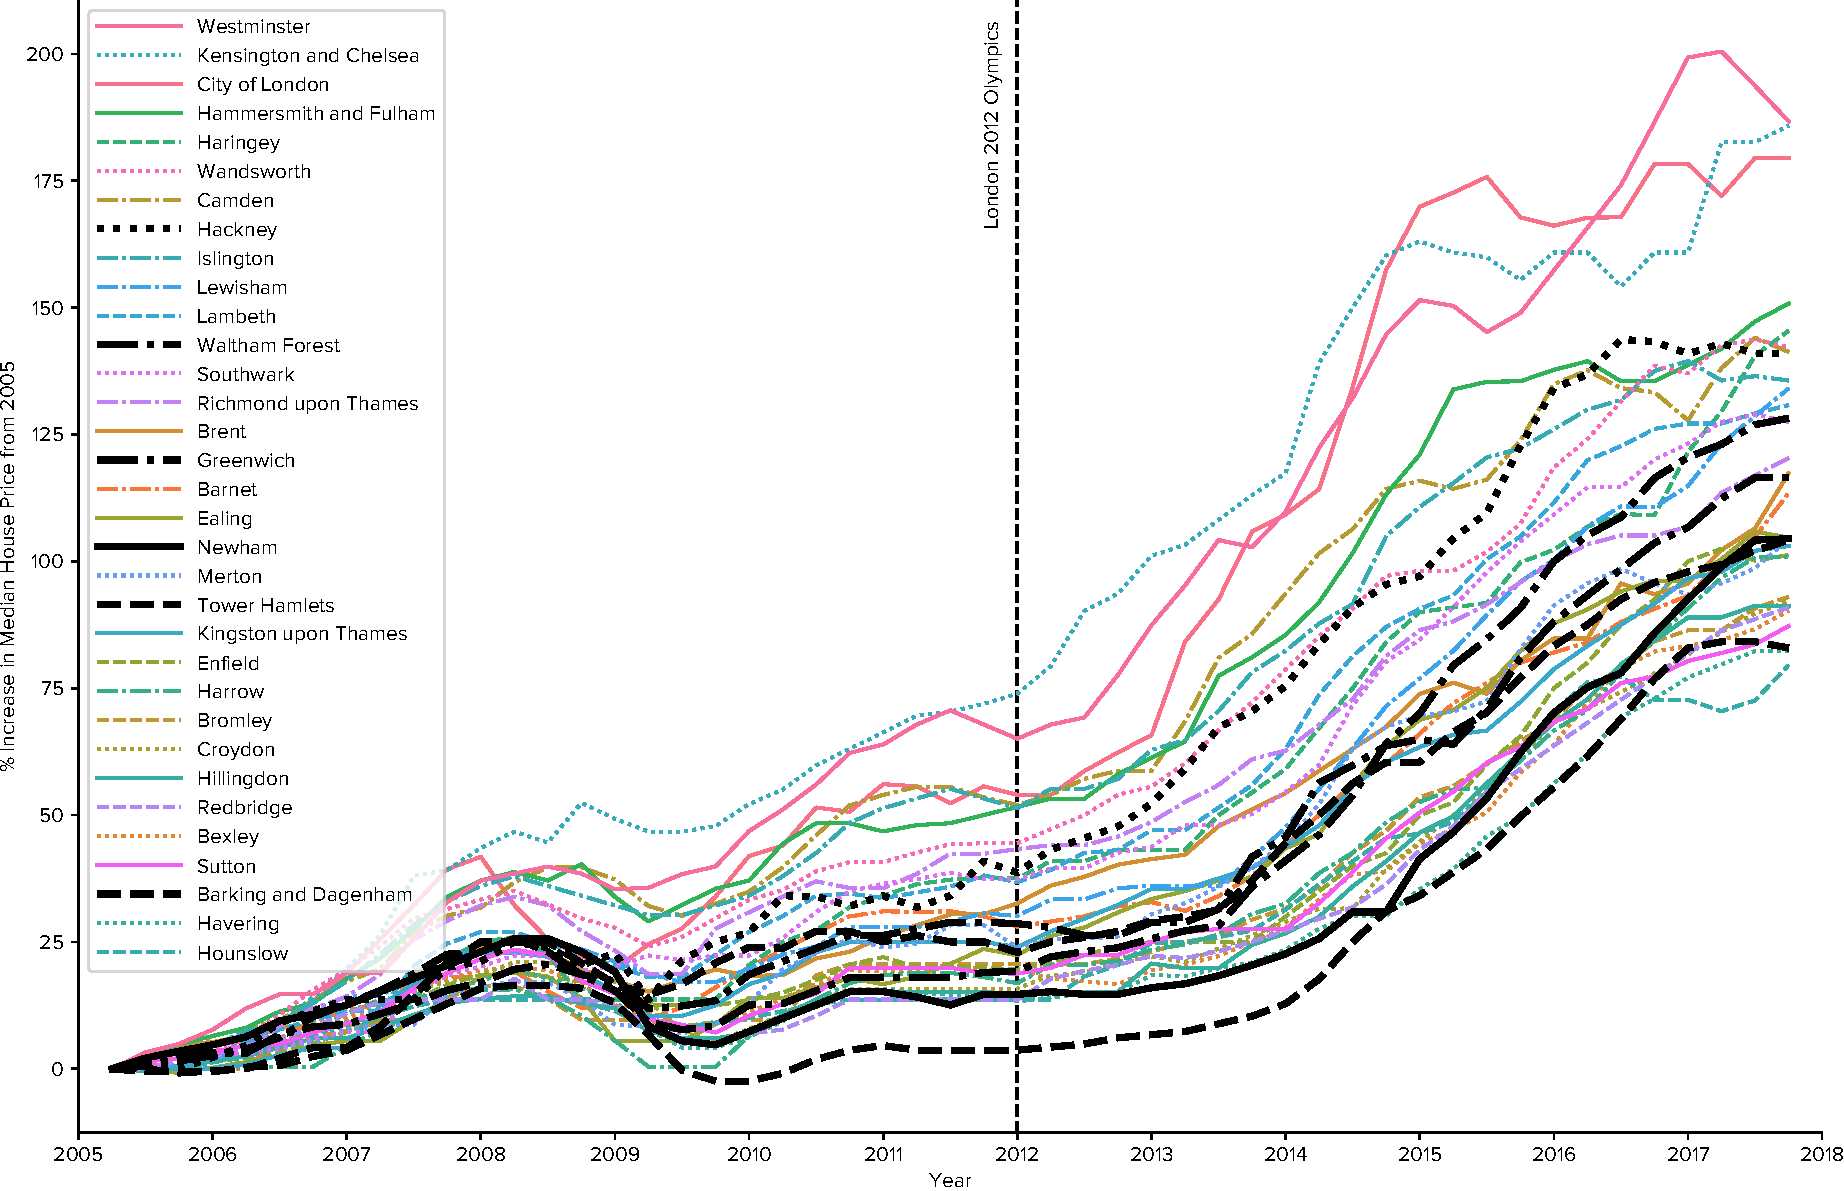
\includegraphics[width=0.8\linewidth]{figures/house-price-percent-change-boroughs.pdf}
\caption{Percent increase in house price in London boroughs from 2005 to 2018.}
\label{fig:house-price-percent-change-boroughs}
\end{figure}

\begin{figure}[!htb]
\centering
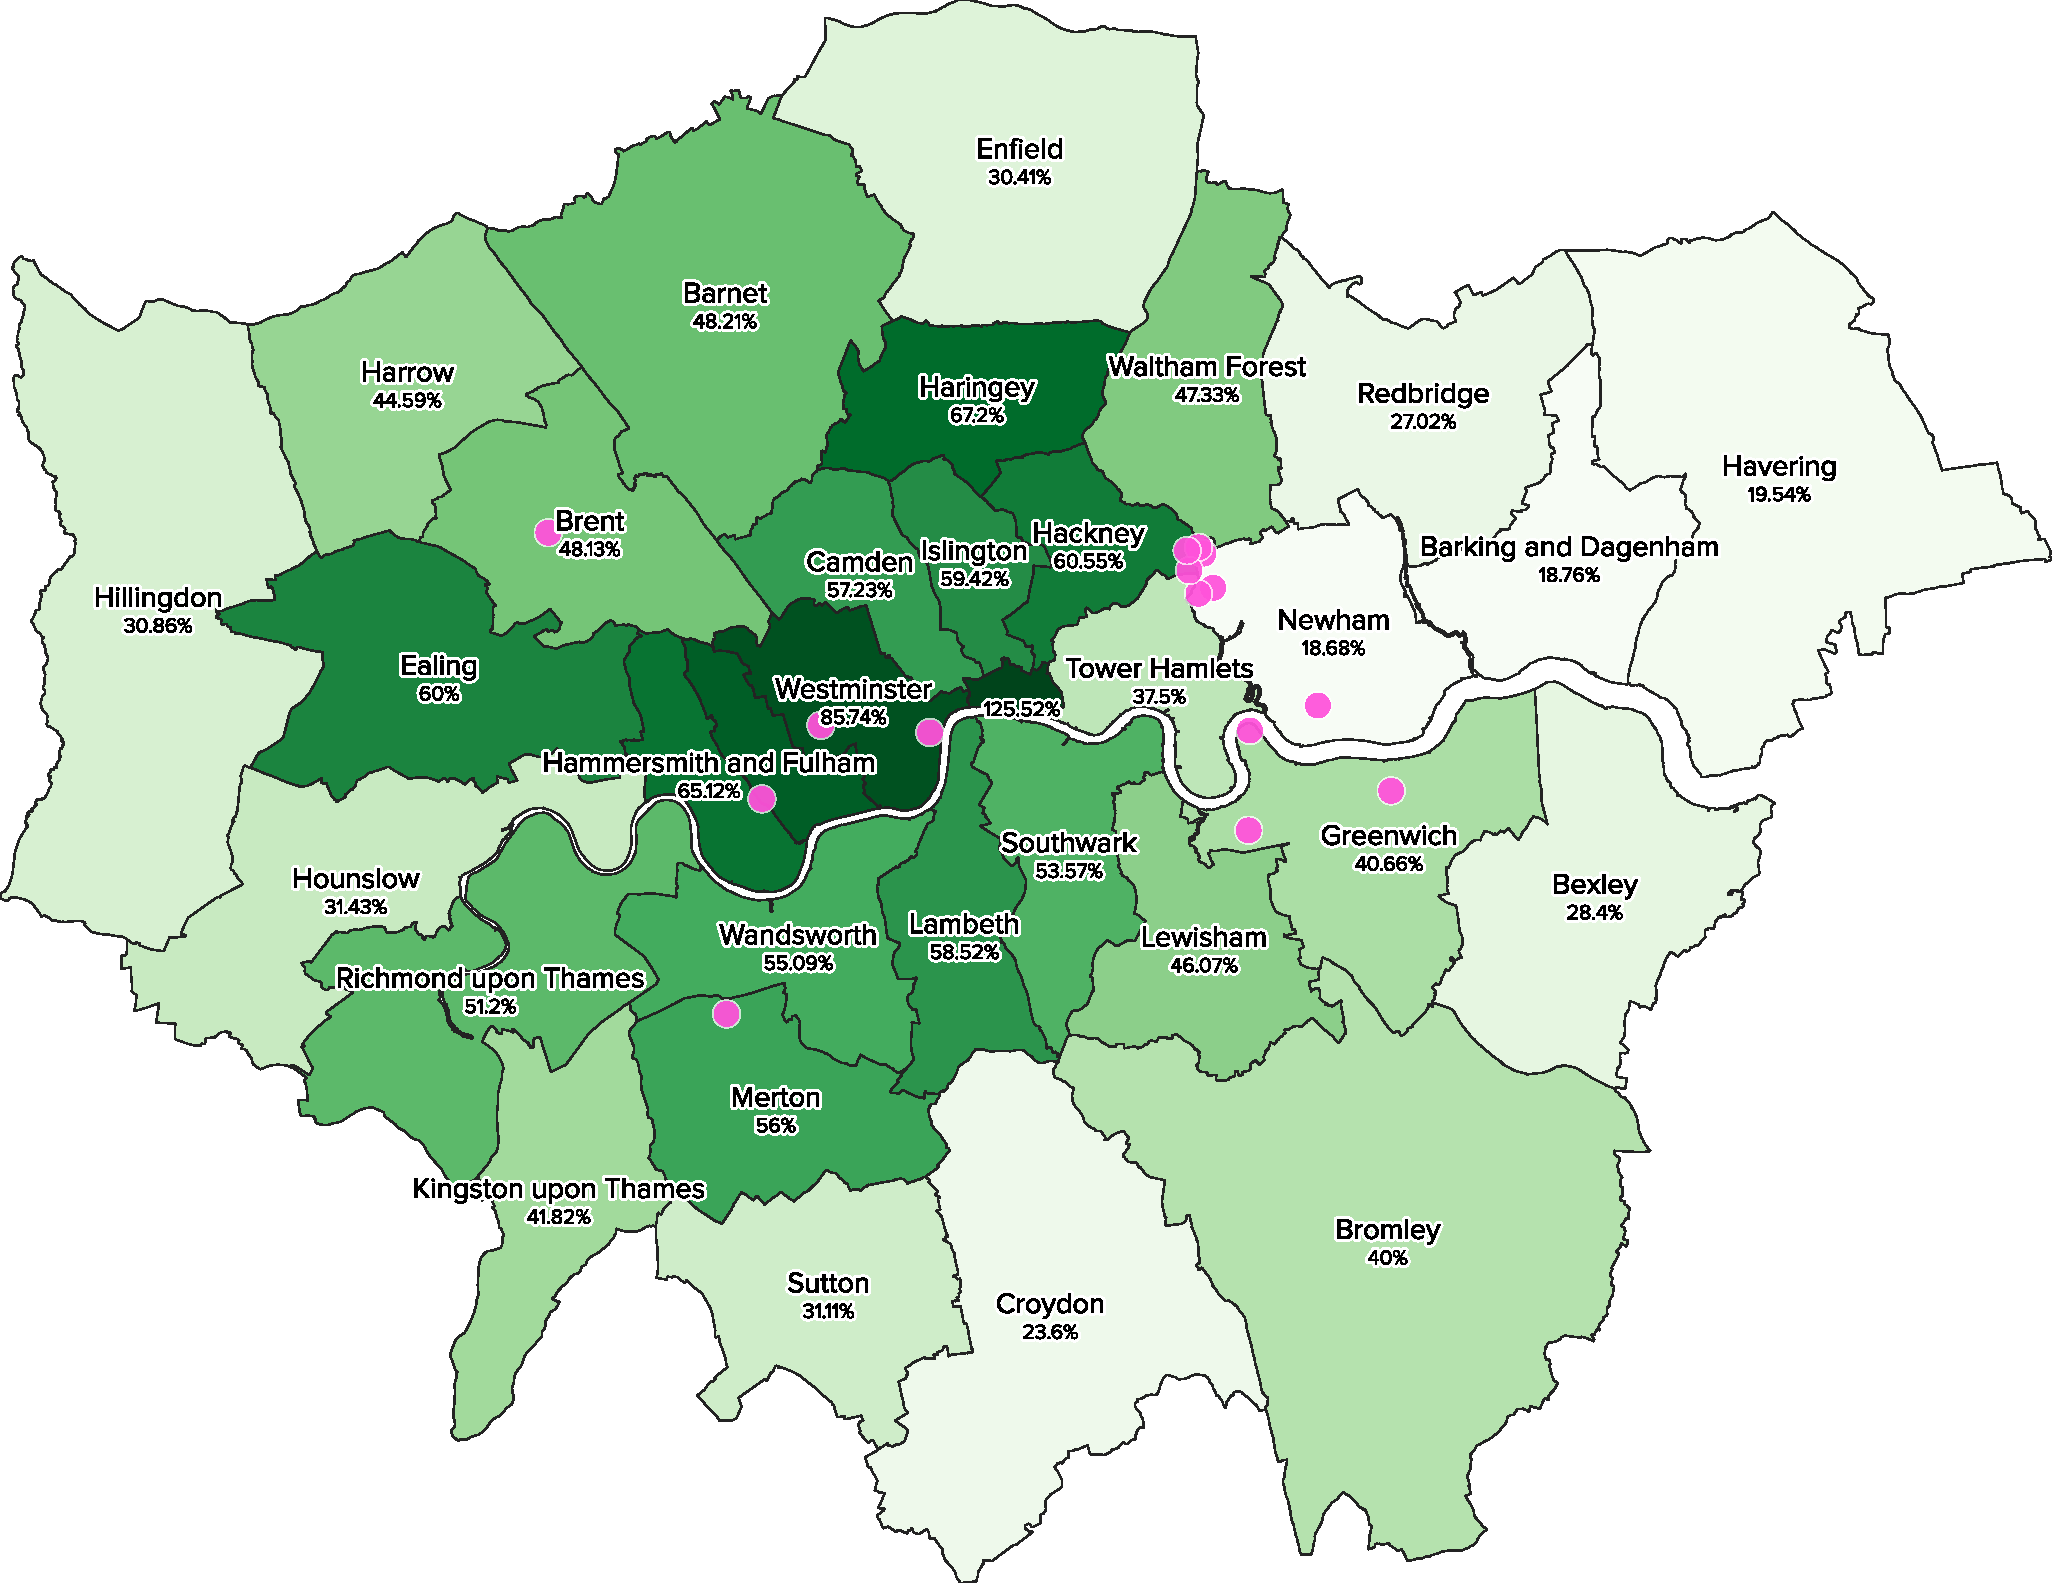
\includegraphics[width=0.8\linewidth]{figures/house-prices-percent-change-borough.pdf}
\caption{Map of London showing the percent increase in house price in each borough from 2009 to 2015, with Olympic venues represented as pink dots.}
\label{fig:house-prices-percent-change-borough-map}
\end{figure}

\begin{figure}[!htb]
\centering
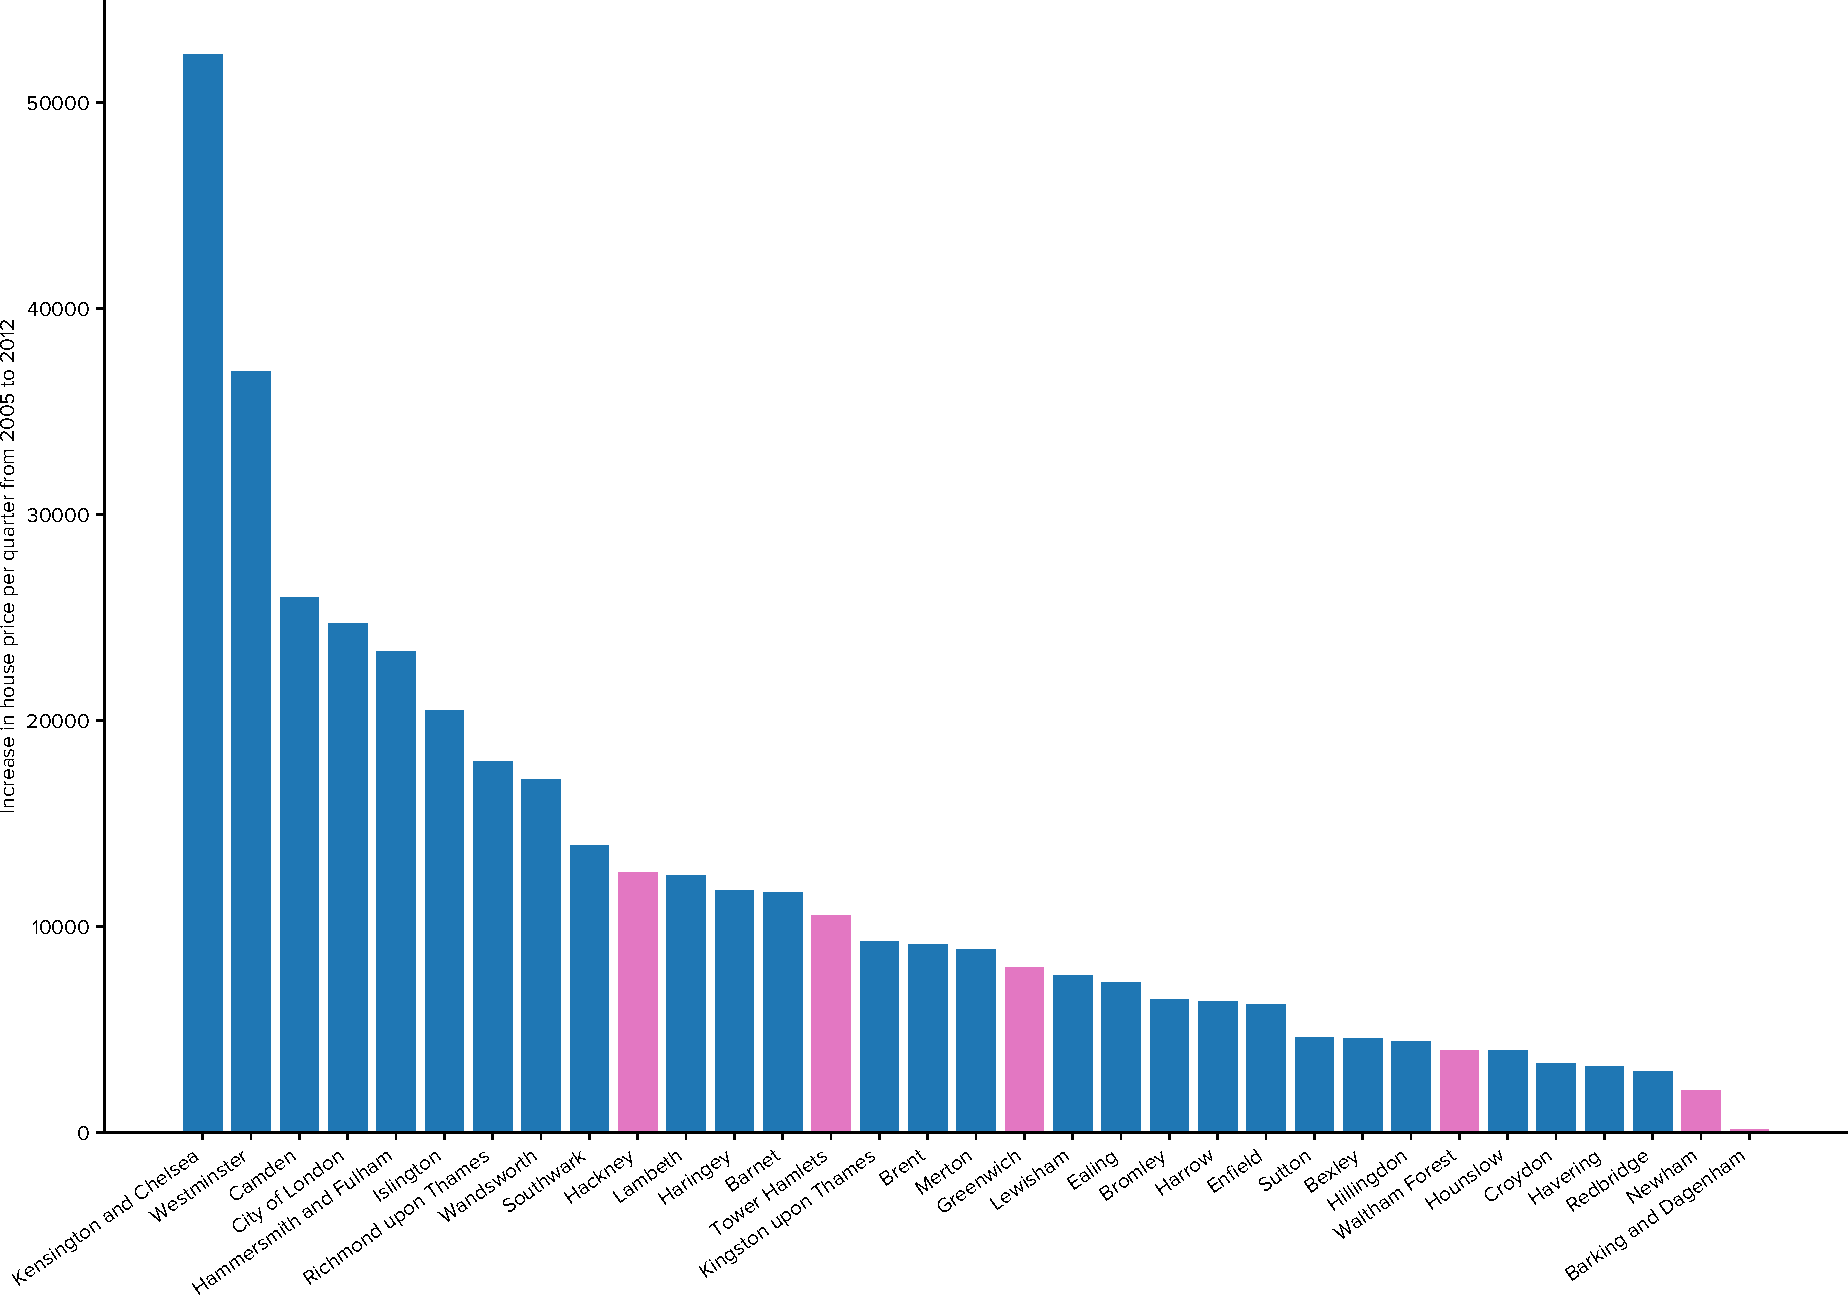
\includegraphics[width=0.8\linewidth]{figures/house-price-trend-before-olympics.pdf}
\caption{Increase in house price per quarter for each borough from 2005 to 2012, in the build-up to the games, based on a linear fit of the data, with host boroughs in pink.}
\label{fig:house-price-trend-before-olympics}
\end{figure}

\begin{figure}[!htb]
\centering
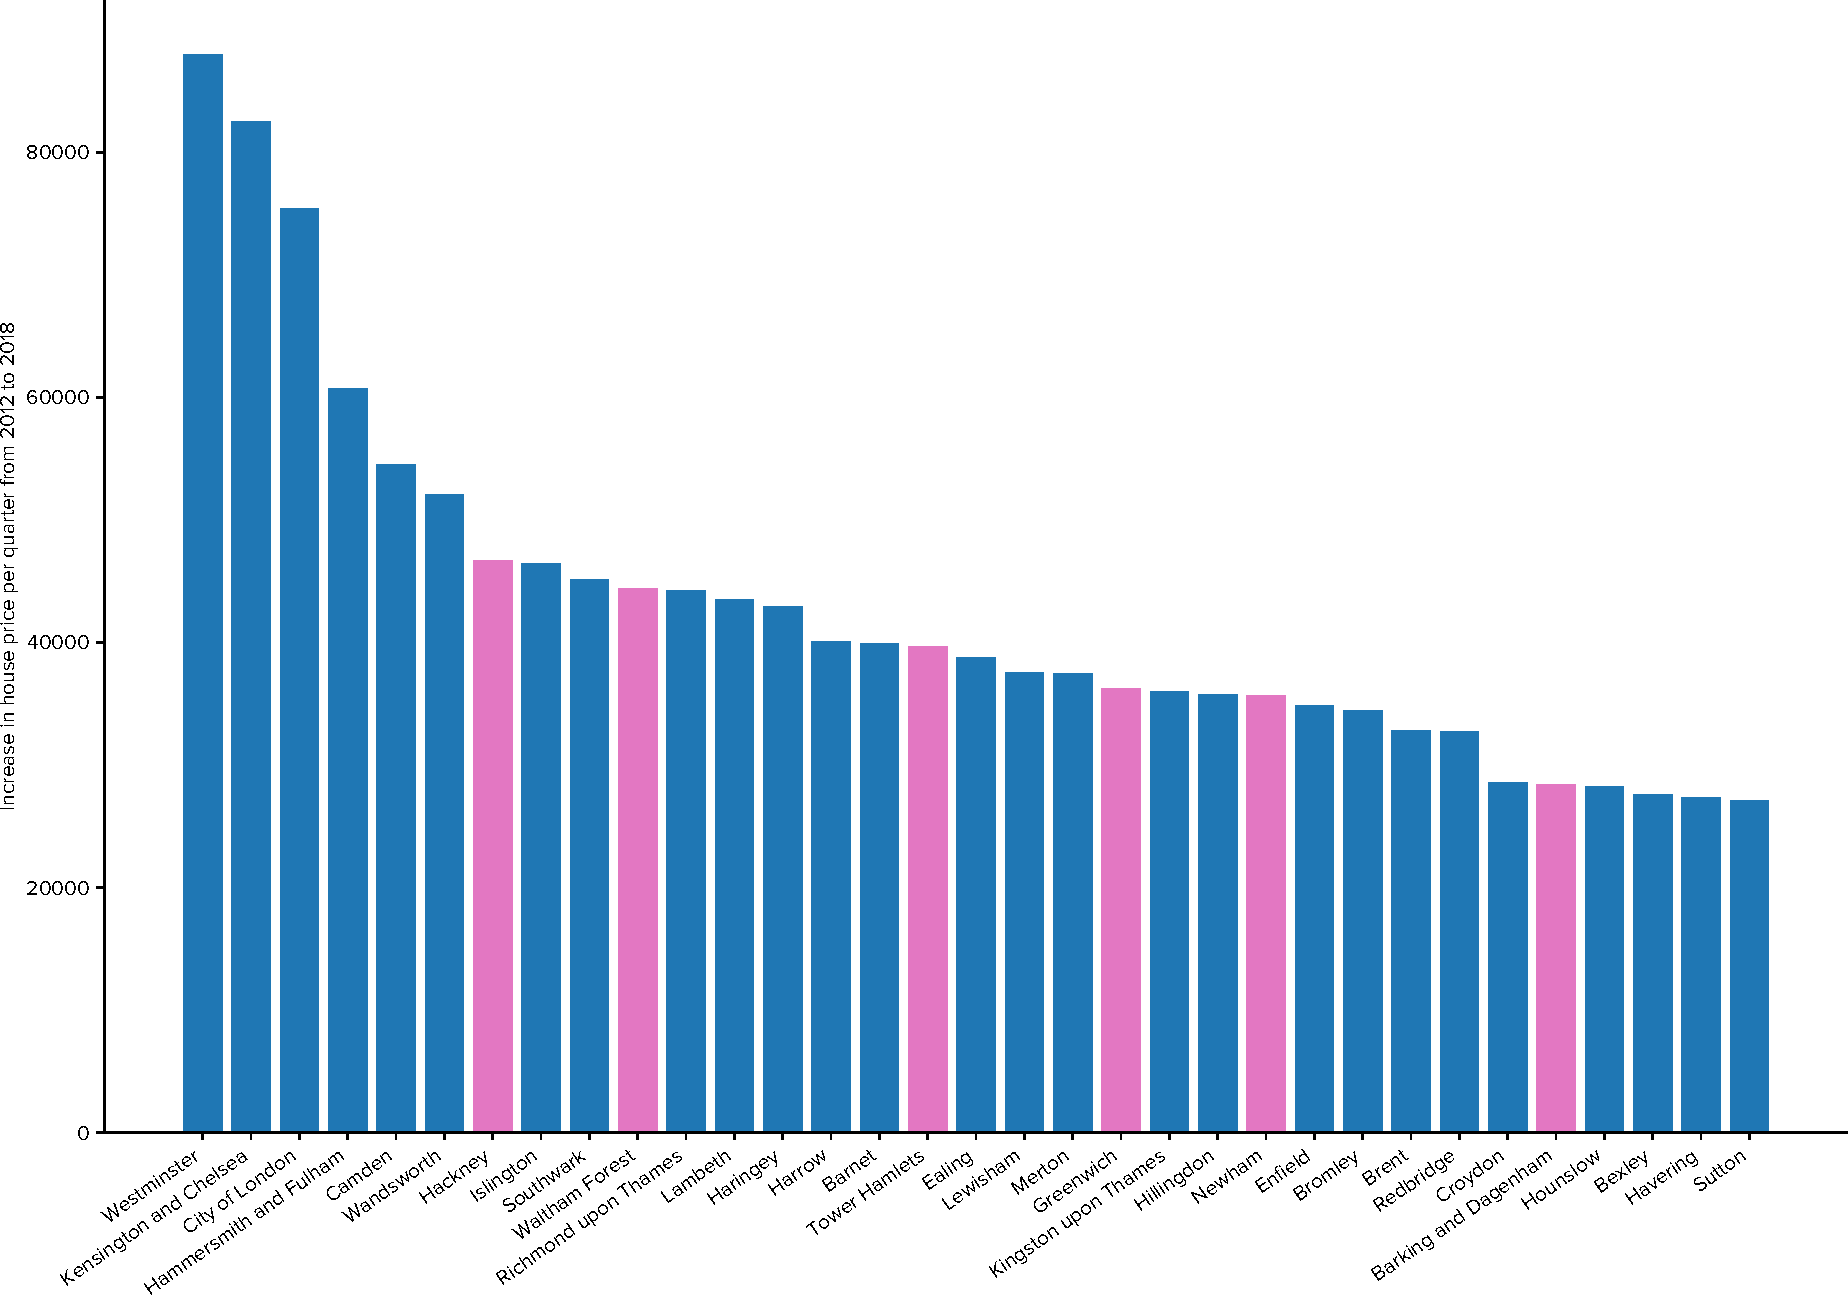
\includegraphics[width=0.8\linewidth]{figures/house-price-trend-after-olympics.pdf}
\caption{Increase in house price per quarter for each borough from 2012 to 2018, after the games, based on a linear fit of the data, with host boroughs in pink.}
\label{fig:house-price-trend-after-olympics}
\end{figure}

\begin{figure}[!htb]
\centering
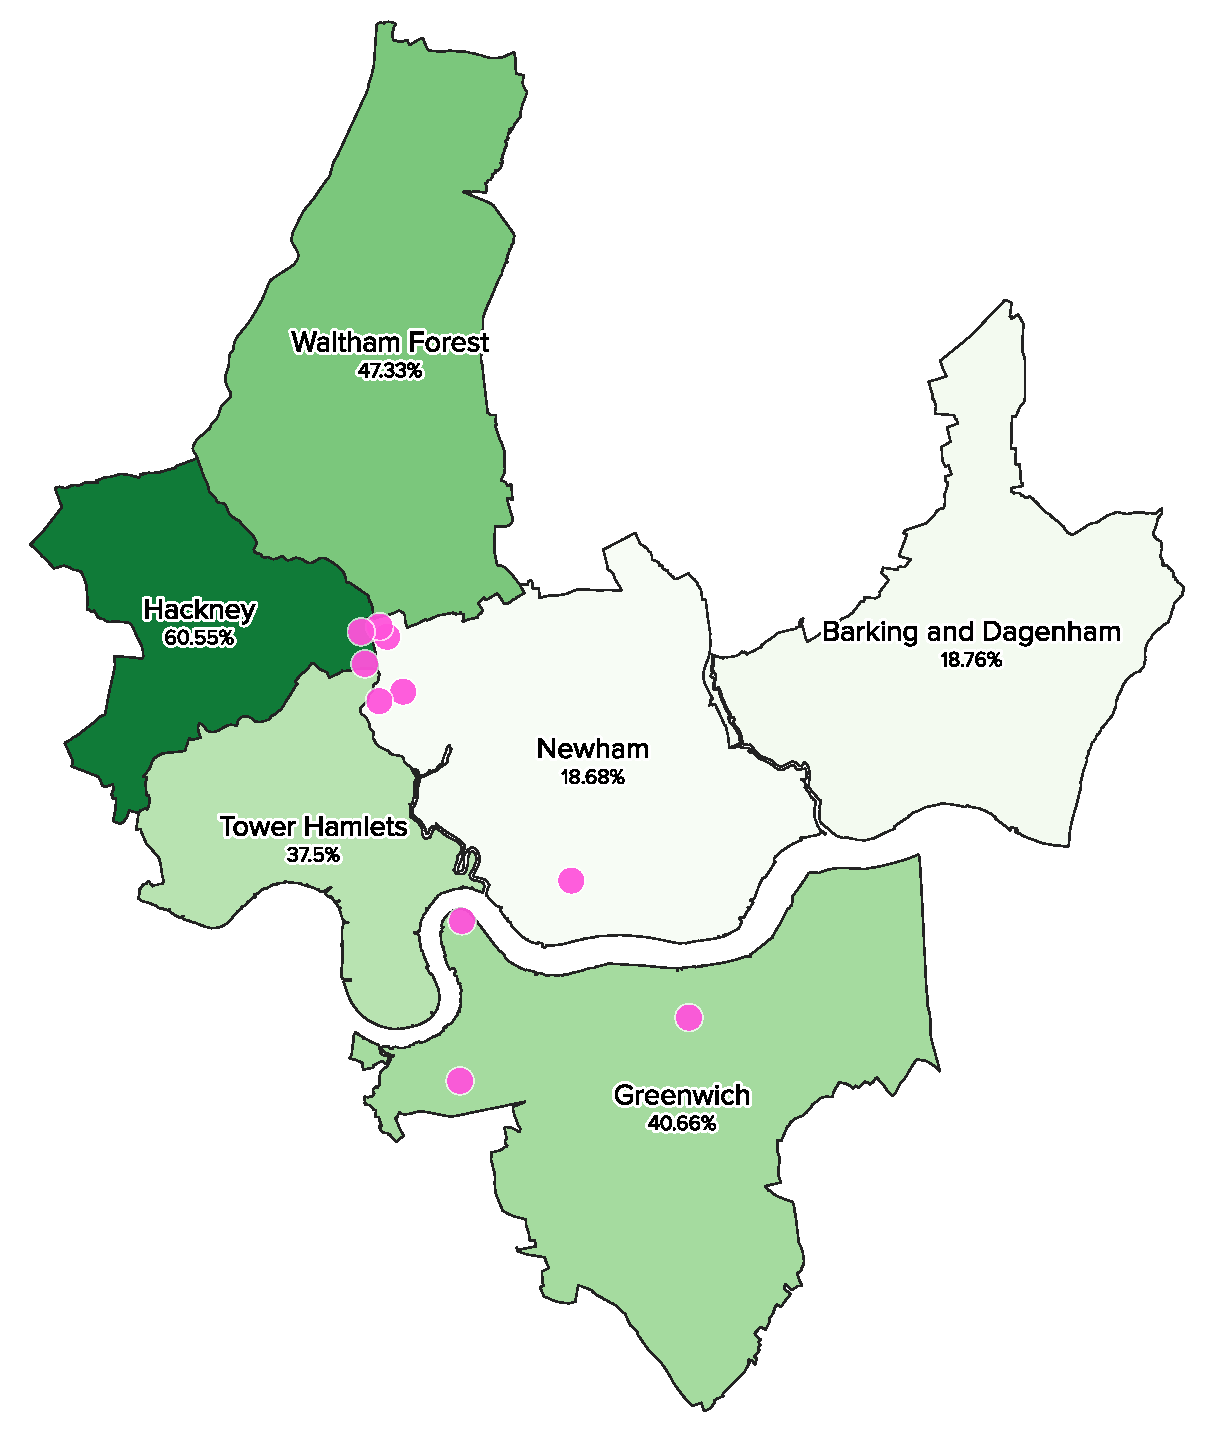
\includegraphics[width=0.6\linewidth]{figures/house-prices-percent-change-growth-boroughs.pdf}
\caption{Map showing the percent increase in house price in each host borough from 2009 to 2015, with Olympic venues represented as pink dots.}
\label{fig:house-prices-percent-change-growth-boroughs-map}
\end{figure}

\begin{figure}[!htb]
\centering
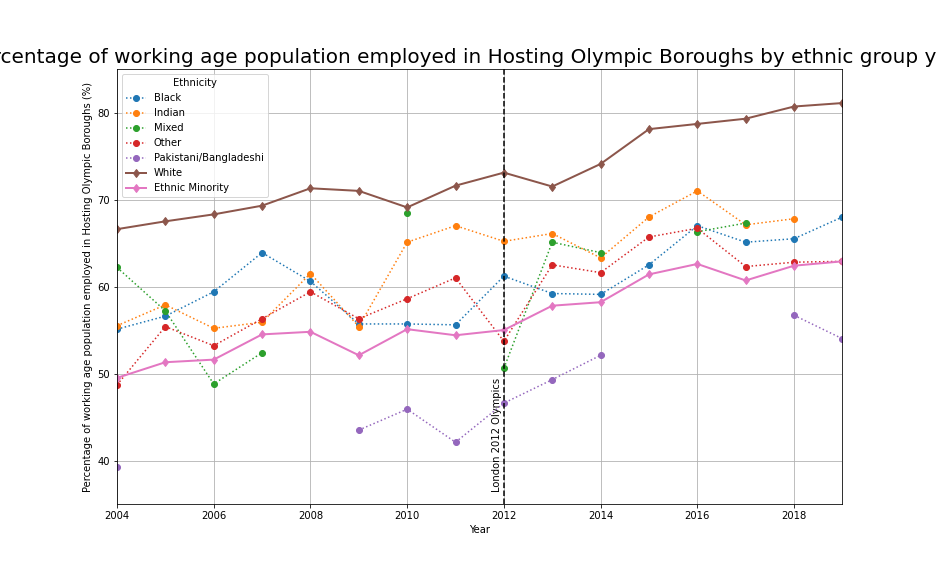
\includegraphics[width=0.9\linewidth]{figures/percentages-Hosting Olympic Boroughs.png}
\caption{Percentage of working age population employed in the hosting Olympic boroughs by ethnic group yearly.}
\label{fig:perc-hosting}
\end{figure}
\begin{figure}[!htb]
\centering
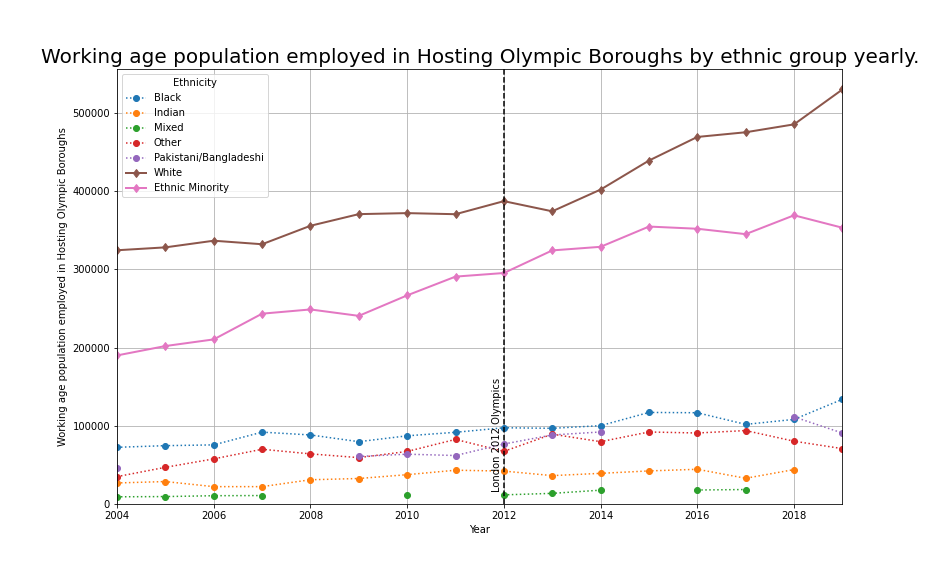
\includegraphics[width=0.9\linewidth]{figures/population-Hosting Olympic Boroughs.png}
\caption{Population of working age population employed in the hosting Olympic boroughs by ethnic group yearly.}
\label{fig:pop-hosting}
\end{figure}

\begin{figure}[!htb]
\centering
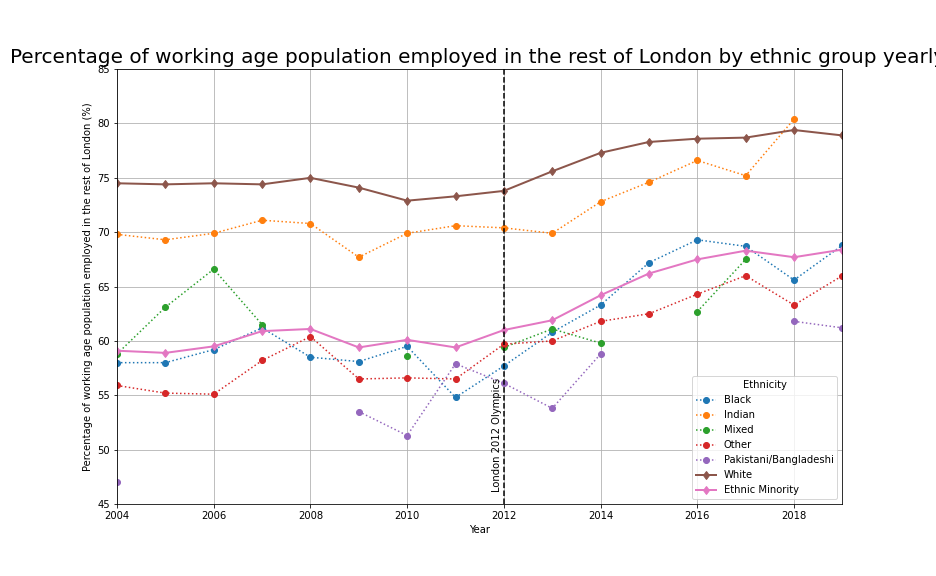
\includegraphics[width=0.9\linewidth]{figures/percentages-the rest of London.png}
\caption{Percentage of working age population employed in London excluding the Olympic boroughs by ethnic group yearly.}
\label{fig:perc-rest-of-london}
\end{figure}
\begin{figure}[!htb]
\centering
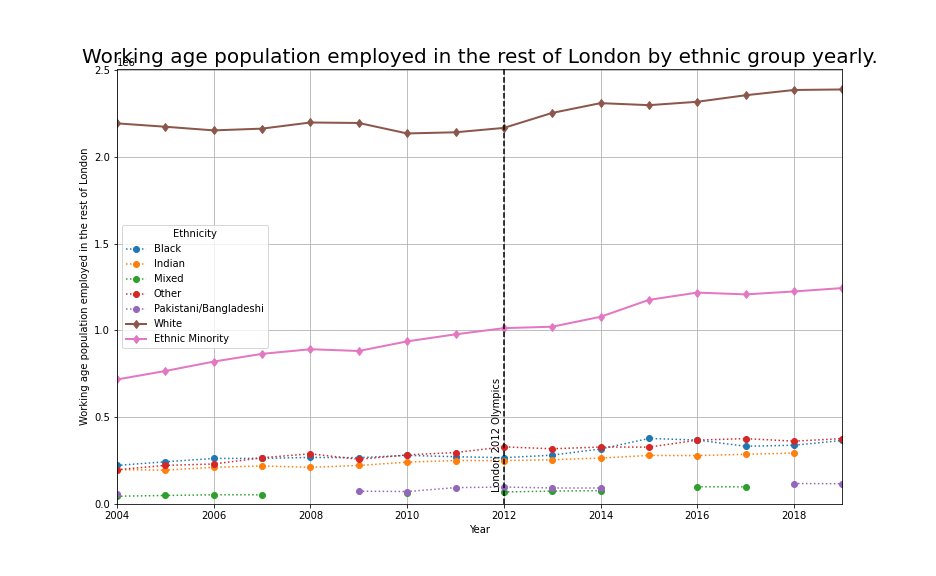
\includegraphics[width=0.9\linewidth]{figures/population-the rest of London.png}
\caption{Population (in millions) of working age population employed in London excluding the Olympic boroughs by ethnic group yearly.}
\label{fig:pop-rest-of-london}
\end{figure}

\begin{figure}[!htb]
\centering
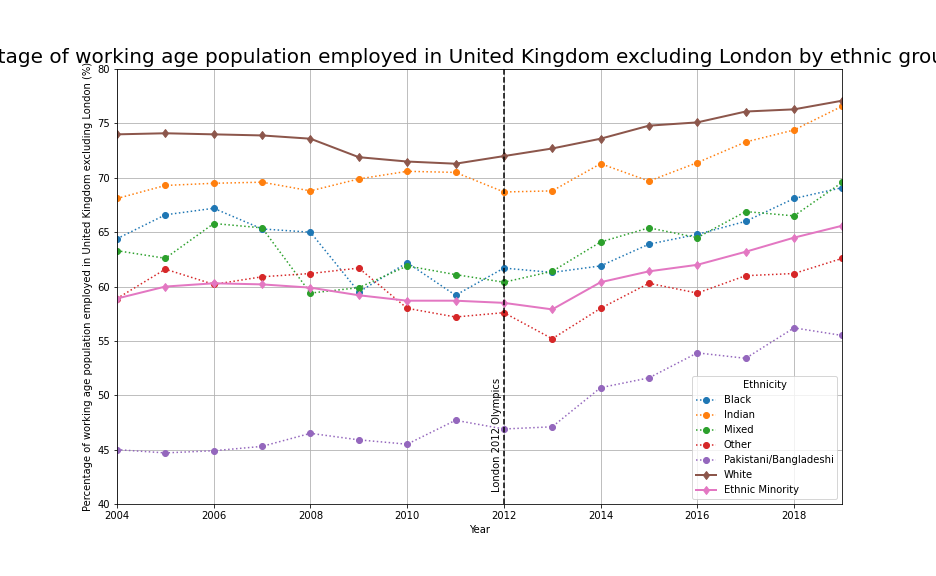
\includegraphics[width=0.9\linewidth]{figures/percentages-United Kingdom excluding London.png}
\caption{Percentage of working age population employed in the UK excluding London by ethnic group yearly.}
\label{fig:perc-uk-no-london}
\end{figure}
% \begin{figure}[!htb]
% \centering
% 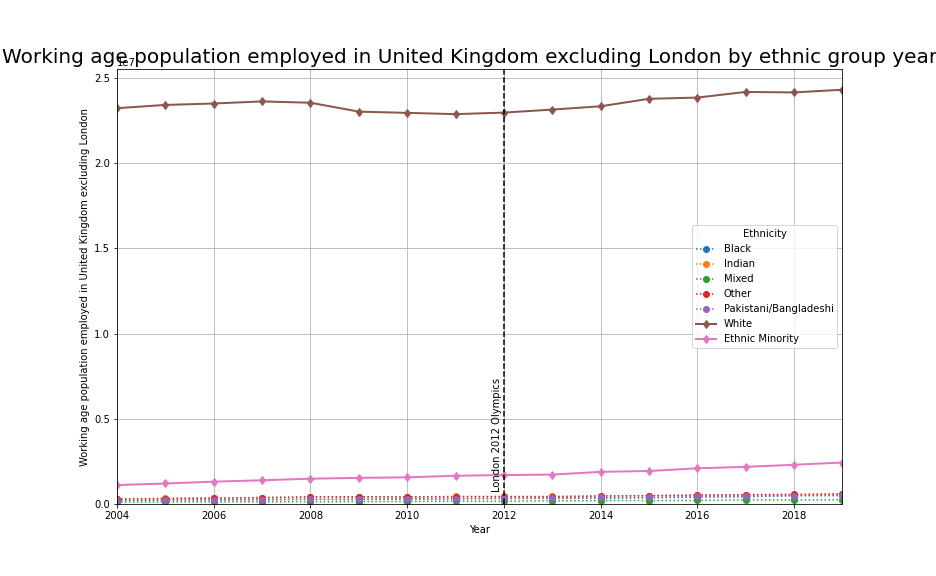
\includegraphics[width=0.9\linewidth]{figures/population-United Kingdom excluding London.png}
% \caption{Population of working age population employed in London excluding the Olympic boroughs by ethnic group yearly.}
% \label{fig:pop-uk-no-london}
% \end{figure}

% \begin{figure}[!htb]
% \centering
% 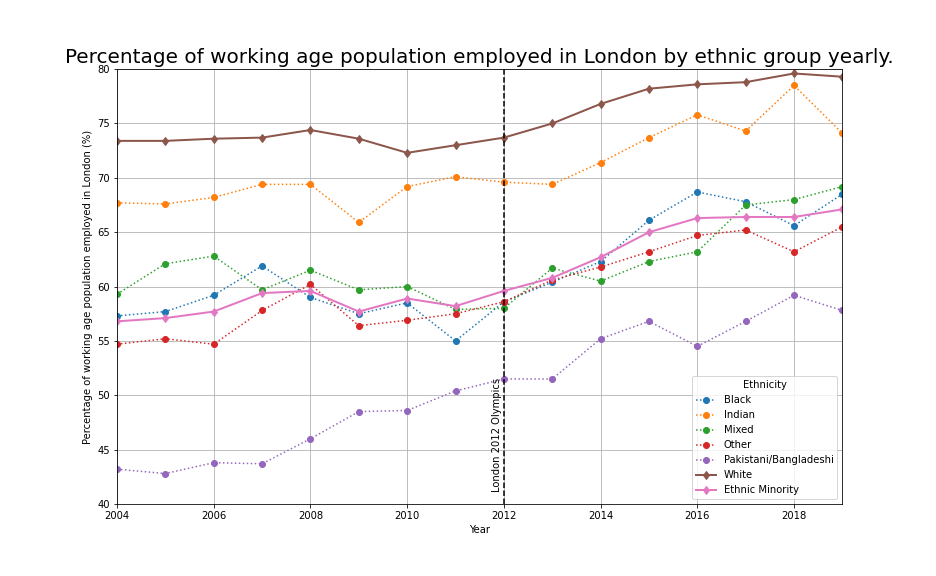
\includegraphics[width=0.9\linewidth]{figures/percentages-London.png}
% \caption{Population of working age population employed in London by ethnic group yearly.}
% \label{fig:perc-london}
% \end{figure}
% \begin{figure}[!htb]
% \centering
% 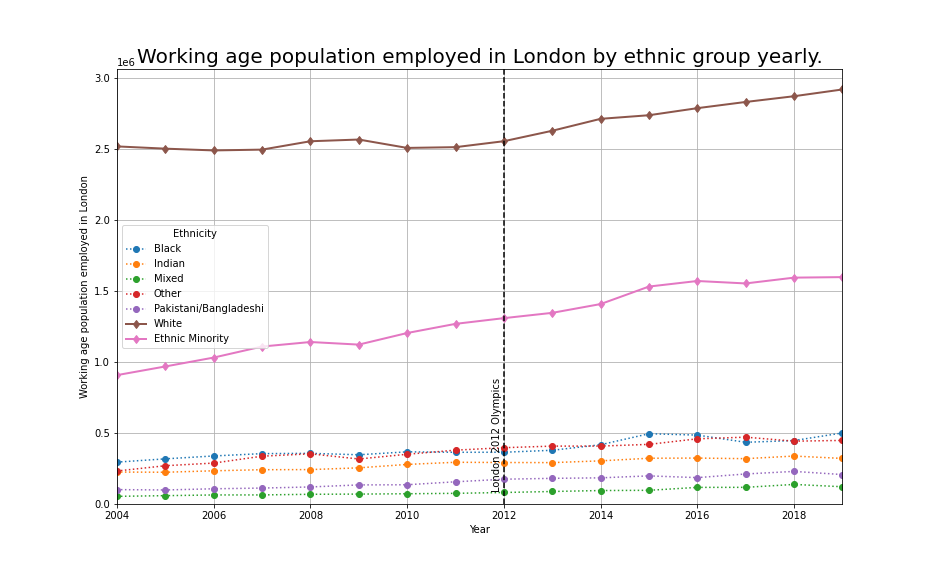
\includegraphics[width=0.9\linewidth]{figures/population-London.png}
% \caption{Population of working age population employed in London by ethnic group yearly.}
% \label{fig:pop-london}
% \end{figure}

% \begin{figure}[!htb]
% \centering
% 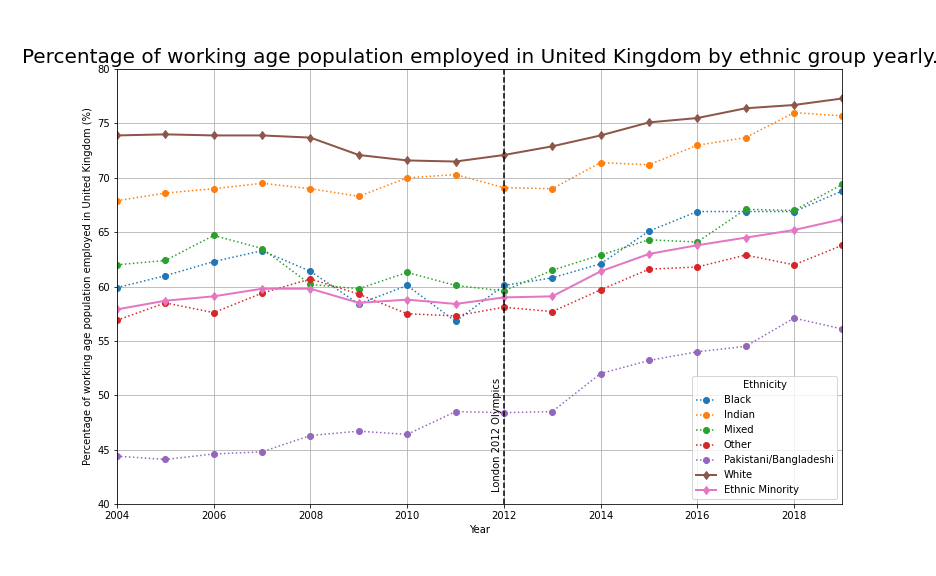
\includegraphics[width=0.9\linewidth]{figures/percentages-United Kingdom.png}
% \caption{Population of working age population employed in the UK by ethnic group yearly.}
% \label{fig:perc-uk}
% \end{figure}
% \begin{figure}[!htb]
% \centering
% 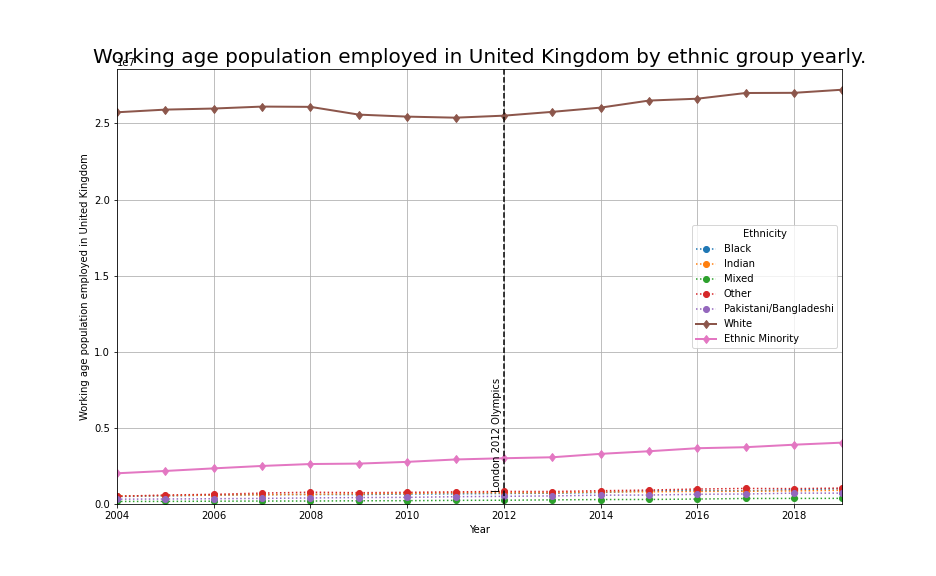
\includegraphics[width=0.9\linewidth]{figures/population-United Kingdom.png}
% \caption{Population of working age population employed in the UK by ethnic group yearly.}
% \label{fig:pop-uk}
% \end{figure}










\end{document}
%%% Local Variables: 
%%% mode: latex
%%% TeX-master: t
%%% End: 
